\documentclass[10pt]{article}\usepackage[correction]{exemptty}
%\documentclass[10pt]{article}\usepackage[enonce]{exemptty}

\TDnumber{9}
\TDmodule{C Seconde Langue}

\usepackage{url,moreverb,wasysym}
\usepackage[utf8]{inputenc}
\hypersetup{colorlinks=false,pdfborder={0 0 0}}

\sloppy
\begin{document}
\title{TP6: L'univers impitoyable des pointeurs}
\maketitle

\newcommand{\I}{\hspace{1.5em}}

\textit{Chances are the baby's yours. I've been just as faithful to our
  marriage vows as you have been, darling.} ~~~ ~~~~~~ \null\hfill--- Sue Ellen
to J.R.

\bigskip

\PseudoExo{Objectifs pédagogiques.}
À la fin de ce TP vous saurez:
\begin{itemize}
\item Manipuler les pointeurs en C
\item Modéliser un problème sous forme de pseudo-objets C (des pointeurs sur
  structure) 
\item Débugger des problèmes d'allocation mémoire (aidez-vous de valgrind et gdb)
\item Comprendre les séries télés d'un autre âge
\end{itemize}
\bigskip

\PseudoExo{Introduction}

On a retrouvé à la mairie de la petite ville américaine de Southfork Ranch un
registre de déclaration des naissances au contenu pour le moins sommaire:

\begin{center}
  \texttt{
    \begin{tabular}[c]{l @{~;~} l @{~;~} l}
      JR Ewing Jr. & Jock Ewing & Miss Ellie \\
%
      Gary Ewing & Jock Ewing & Miss Ellie \\
      Bobby Ewing & Jock Ewing & Miss Ellie \\
      Tina Ewing & JR Ewing Jr. & Sue Ellen Shepard \\
      JR Ewing III & JR Ewing Jr. & Sue Ellen Shepard \\
%
      Lucy Ewing & Garry Ewing & Valene Clements \\
      Christopher Ewing & Bobby Ewing & Pamela Barnes \\
      Ray Krebbs& Jock Ewing& Margaret Hunter\\
      Margaret Krebbs & Ray Krebbs & Donna Culver\\     
      Lucas Ewing & Ray Krebbs & Jenna Wade\\     
    \end{tabular}
  }
\end{center}

Après un gros effort de recherche, on a fini par comprendre l'histoire de ces
personnes, bientôt relatée dans un feuilleton qui déchaîne les passions du
monde tout entier.

Si vous avez raté les 5683 premiers épisodes, consultez votre magazine télé
préféré qui vous résume l'histoire (en «s'inspirant» honteusement de Wikipédia):

\emph{Jock et Miss Ellie ont eu trois fils, J.R., Gary et Bobby. J.R., le fils
  Ewing aîné sans scrupule était marié sans amour à une ancienne Miss Texas,
  Sue Ellen Shepard Ewing. Il était fréquemment en conflit avec son plus jeune
  frère, Bobby, garant de la morale et l'intégrité qui manquait tant à son
  frère aîné. Gary, le second fils, était le mouton noir de la
  famille. Longtemps mal aimé de Jock et mal traité par J.R., il eut une
  relation profonde quoique distante avec Bobby et Ellie. Il s'est marié avec
  Valene "Val" Clements Ewing, qui mis au monde une fille, Lucy, la nièce
  impertinente mais compliquée de J.R. et Bobby. Elle passa la plus grande
  partie de sa vie à Southfork avec ses grands-parents. Elle eut une affaire
  avec le contremaître du ranch Ray Krebbs. Ray s'avéra être son demi-frère,
  issu d'une aventure extra-conjugale de Jock avec Margaret Hunter, une
  infirmière rencontrée par Jock pendant la seconde guerre mondiale.  Ray se
  maria finalement avec Donna Culver, et une enfant du nom de Margaret Krebbs
  naquit de leur union, bien que le divorce fut prononcé bientôt. Plus tard,
  Ray se maria à Jenna Wade, qui donna bientôt naissance à un petit Lucas.}

En attendant l'épisode suivant, vous avez déjà traduit l'histoire par
le graphe présenté plus loin.

\Exercice\textbf{Comprendre le problème.}

Entre deux épisodes, vous décidez de développer un outil informatique qui vous
permettra de suivre en temps réel les évolutions démographiques des 63521
épisodes restants. Pour cela vous résoudrez les problèmes suivants.

\Question Que signifient 6 références de chaque nœud dans le graphe suivant?

\begin{Reponse}
  Dans le sens des aiguilles d'une montre, en partant d'en haut à gauche.
  \begin{itemize}
  \item Père
  \item Mère
  \item Frère ou demi-frère par le père (ou sœur)
  \item Frère ou demi-frère par la mère (ou sœur)
  \item L'un des enfants
  \item Chaînage contenant tous les nœuds existants
  \end{itemize}

\end{Reponse}

\Question À quoi sert le chaînage général de tous les nœuds (celui en
pointillés) ?

\begin{Reponse}
  Il contient donc tous les éléments de la structure. Ca peut être utile pour
  chercher une personne d'après son nom, par exemple.
\end{Reponse}

\Question Quel est l'intérêt des chaînages cycliques horizontaux de ce graphe ?

\begin{Reponse}
  Il s'agit donc des liens de fraterie. Il faut couper en deux car il y a une
  fraterie par le père, et une fraterie par la mère.
\end{Reponse}

Tant que vous n'avez pas compris les liens entre l'histoire, le registre et le
graphe, n'allez pas plus loin et recommencez cet exercice.


\Exercice\textbf{Réalisation de la structure correspondante.}

\Question Écrivez la structure décrivant une personne. Nous allons l'utiliser
comme pseudo-classe en C.
\begin{Reponse}
  \begin{Verbatim}[gobble=4]
    typedef struct node {
      struct node *pere;
      struct node *mere;
      struct node *frere_pere;
      struct node *frere_mere;
      struct node *enfant;
      struct node *next;
      char *nom;
      int ismale;
    } node;
  \end{Verbatim}
\end{Reponse}

\Question Écrivez le constructeur de cette classe qui prendra comme argument le
nom de la personne et son sexe. Ce nouveau nœud du graphe sera pour l'instant
considéré comme n'ayant pas de parents, ni frère ni sœur (comme Jock dans
l'exemple). On pourra considérer qu'il n'existe pas 2 personnes portant le même
nom.

\begin{Reponse}
  \begin{Verbatim}[gobble=4]
    node *node_create(char *name, int ismale) {
      node *res=malloc(sizeof(struct node));
      strcpy(res->name,name);
      res->ismale = ismale;
      res->pere = NULL;
      res->mere = NULL;
      res->frere_pere = res; // on boucle sur soi-meme
      res->frere_mere = res; // on boucle sur soi-meme
      res->enfant = NULL;
      res->next=res; // on boucle sur soi-meme
      return res;
    }
  \end{Verbatim}
\end{Reponse}

\Question Écrivez la fonction permettant d'insérer un nouveau nœud dans la
liste de tous les nœuds présents dans le graphe.

\begin{Reponse}
  \begin{Verbatim}[gobble=4]
    node *allnodes=NULL;
    void node_link(node *n) {
      if (allnodes==NULL) {
        allnodes=n;// premier noeud créé. C'est plus simple
      } else {
        // cherchons la fin du cycle (allnodes est la sentinelle)
        node *iterator = allnodes;
        iterator=allnodes;
        while (iterator->next != allnodes)
          iterator = iterator->next;
        // Inserons n à la fin du cycle
        n->next=allnodes;
        iterator->next=n;
      }
    }
  \end{Verbatim}
\end{Reponse}


\Question Écrivez une fonction modifiant différentes références entre nœuds du
graphe, lors de l'établissement d'une filiation père/enfant. Cette fonction
aura deux paramètres: l'objet représentant le père et celui représentant
l'enfant.
\begin{Reponse}
  \begin{Verbatim}[gobble=4]
    void node_change_pere(node *pere,node*fils) {
      if (pere->fils) { // il y a deja des enfants
        // Cherchons le dernier fils (en utilisant pere->fils comme sentinelle)
        node *last = pere->fils;
        while (last->frere_pere != pere->fils)
          last = last->frere_pere;
        // On insere le nouveau avant le premier et après last
        fils->frere_pere = pere->fils;
        last->frere_pere = fils;
      } else {
        pere->fils=fils;
        fils->pere=pere;
      }
    }
  \end{Verbatim}
\end{Reponse}


\Question Même question mais lors de l'établissement d'une filiation
mère/enfant.

\begin{Reponse}
  Même genre de réponse (je n'ai rien tenté de compiler de toute façon, c'est
  une correction à l'arrache).
\end{Reponse}

\Question Écrivez une fonction qui prend un nom en paramètre et qui renvoie
l'objet correspondant (ou NULL si le nom n'existe pas dans le graphe).

\begin{Reponse}
  \begin{Verbatim}[gobble=4]
    node*node_by_name(char *name) {
      node *iterator = allnodes;
      do {
        if (!strcmp(iterator->name,name))
          return iterator;
        iterator=iterator->next;
      } while (iterator != allnodes);
      return NULL;
    }
  \end{Verbatim}
\end{Reponse}

\Question Écrivez une fonction qui affiche l'état du graphe à un instant
donné. Vous pouvez par exemple écrire une fonction qui, pour chaque nœud, écrit
sur la sortie standard le nom de la personne et ceux de ses six voisins.

\Question Écrivez une fonction qui lit un registre de naissances et crée le
graphe correspondant.

A cet instant du projet, vous devriez être capables de créer le graphe
correspondant à l'épisode du jour. Vous êtes donc prêts pour les
rebondissements à venir :

\Exercice\textbf{Modifications à la structure} \textit{(attention spoiler!)}

\Question Terrible rebondissement durant l'épisode de cette semaine ! Lucas
n'est pas le fils de Ray, mais de son demi-frère Bobby !! Écrivez une fonction
qui prend en paramètre les noms de l'enfant et du \emph{vrai} père et qui
modifie le graphe en conséquence.

\Question Encore un rebondissement sordide cette semaine: Tina Ewing n'est pas
la fille de J.R. et Sue Ellen. En effet, Sue Ellen ayant eu peur que Pamela
donne un héritier à la famille Ewing avant elle, elle avait acheté un bébé à
une femme. Quand J.R. découvrit l'histoire (dès l'épisode 10), il renvoie le
bébé auprès de sa mère, affirmant à sa femme qu'il veut un enfant autant
qu'elle, mais qu'il doit être «notre enfant, pas celui de quelqu'un d'autre».

Écrivez une fonction qui prend en paramètre les noms de l'enfant et de sa
\emph{vraie} mère et qui modifie le graphe en conséquence.

\Question Suite à ces différentes révélations, écrivez une fonction qui détecte
les éventuelles anomalies généalogiques d'un graphe (avoir son père comme fils
ou comme frère par exemple). Appliquez cette fonction au graphe de l'exemple.

\Question Écrivez une fonction qui affiche les ascendants successifs d'un nœud
(son arbre généalogique donc). Appliquez cette fonction à tous les nœuds du
graphe.

\Question Écrivez une fonction qui affiche les descendants d'un nœud pour une
génération dont le numéro sera passé en second paramètre.

\Question Écrivez une fonction qui affiche les descendants d'un nœud, génération
par génération, jusqu'à une génération passée en second paramètre.

\Exercice\textbf{Aller plus loin.}

\Question Écrivez une fonction qui ordonne le chaînage général du graphe selon
l'ordre alphabétique des noms. Affichez le graphe ainsi obtenu.

\Question Ray est devenu fou. Excédé par les vicicitudes des Ewing, il décide
de tuer tous les membres de la famille (tuant également tout espoir des
producteurs d'une suite possible sur TNT l'an prochain).  Exercez sa vengeance
en exécutant un par un la famille de Jock. Affichez le graphe résultat publié
par la presse après chaque acte de vengeance.

\Question Écrivez la méthode qui sauvegarde la structure de données sur fichier
(on parle de sérialisation).

\Question Écrivez la méthode qui crée le graphe à partir d'un fichier de
sauvegarde produit par la méthode de la question précédente.

\vfill
\hrule

\medskip\noindent
Merci à Dominique Lazure pour l'idée initiale, et Frédéric Suter pour
l'avoir sauvée par delà les âges.

\begin{figure}
  \centering
  \resizebox{.8\linewidth}{!}{\rotatebox{270}{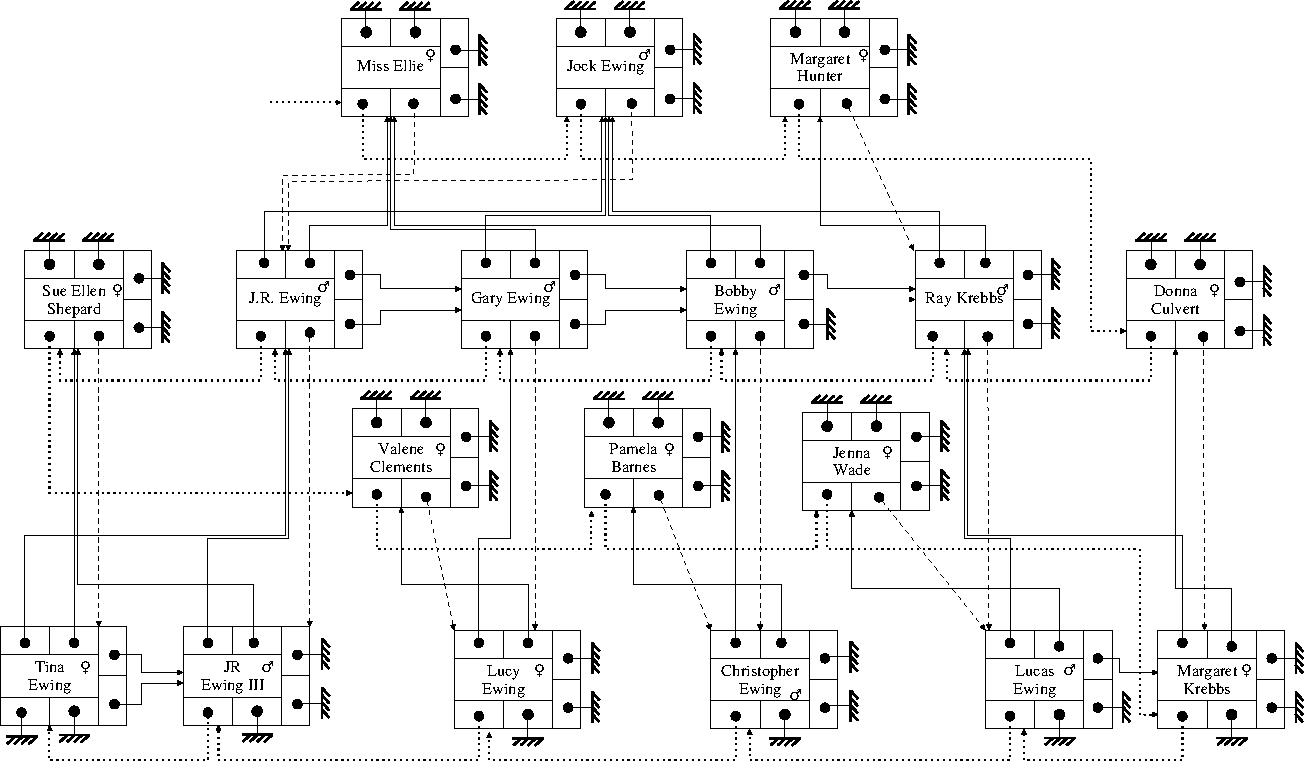
\includegraphics{arbre-genealogique.pdf}}}

\end{figure}

\end{document}
